\section{Thiết kế Logic và Giải pháp Kỹ thuật}

\subsection{Mô hình Kiến trúc Phân cấp (Hierarchical Design)}
Để đảm bảo khả năng mở rộng và dễ dàng quản trị cho Cơ sở Bảo Lộc, nhóm đề xuất mô hình mạng 3 lớp tiêu chuẩn Cisco:

\begin{figure}[H]
    \centering
    % Ảnh được tạo từ script python ve_so_do_logic.py
    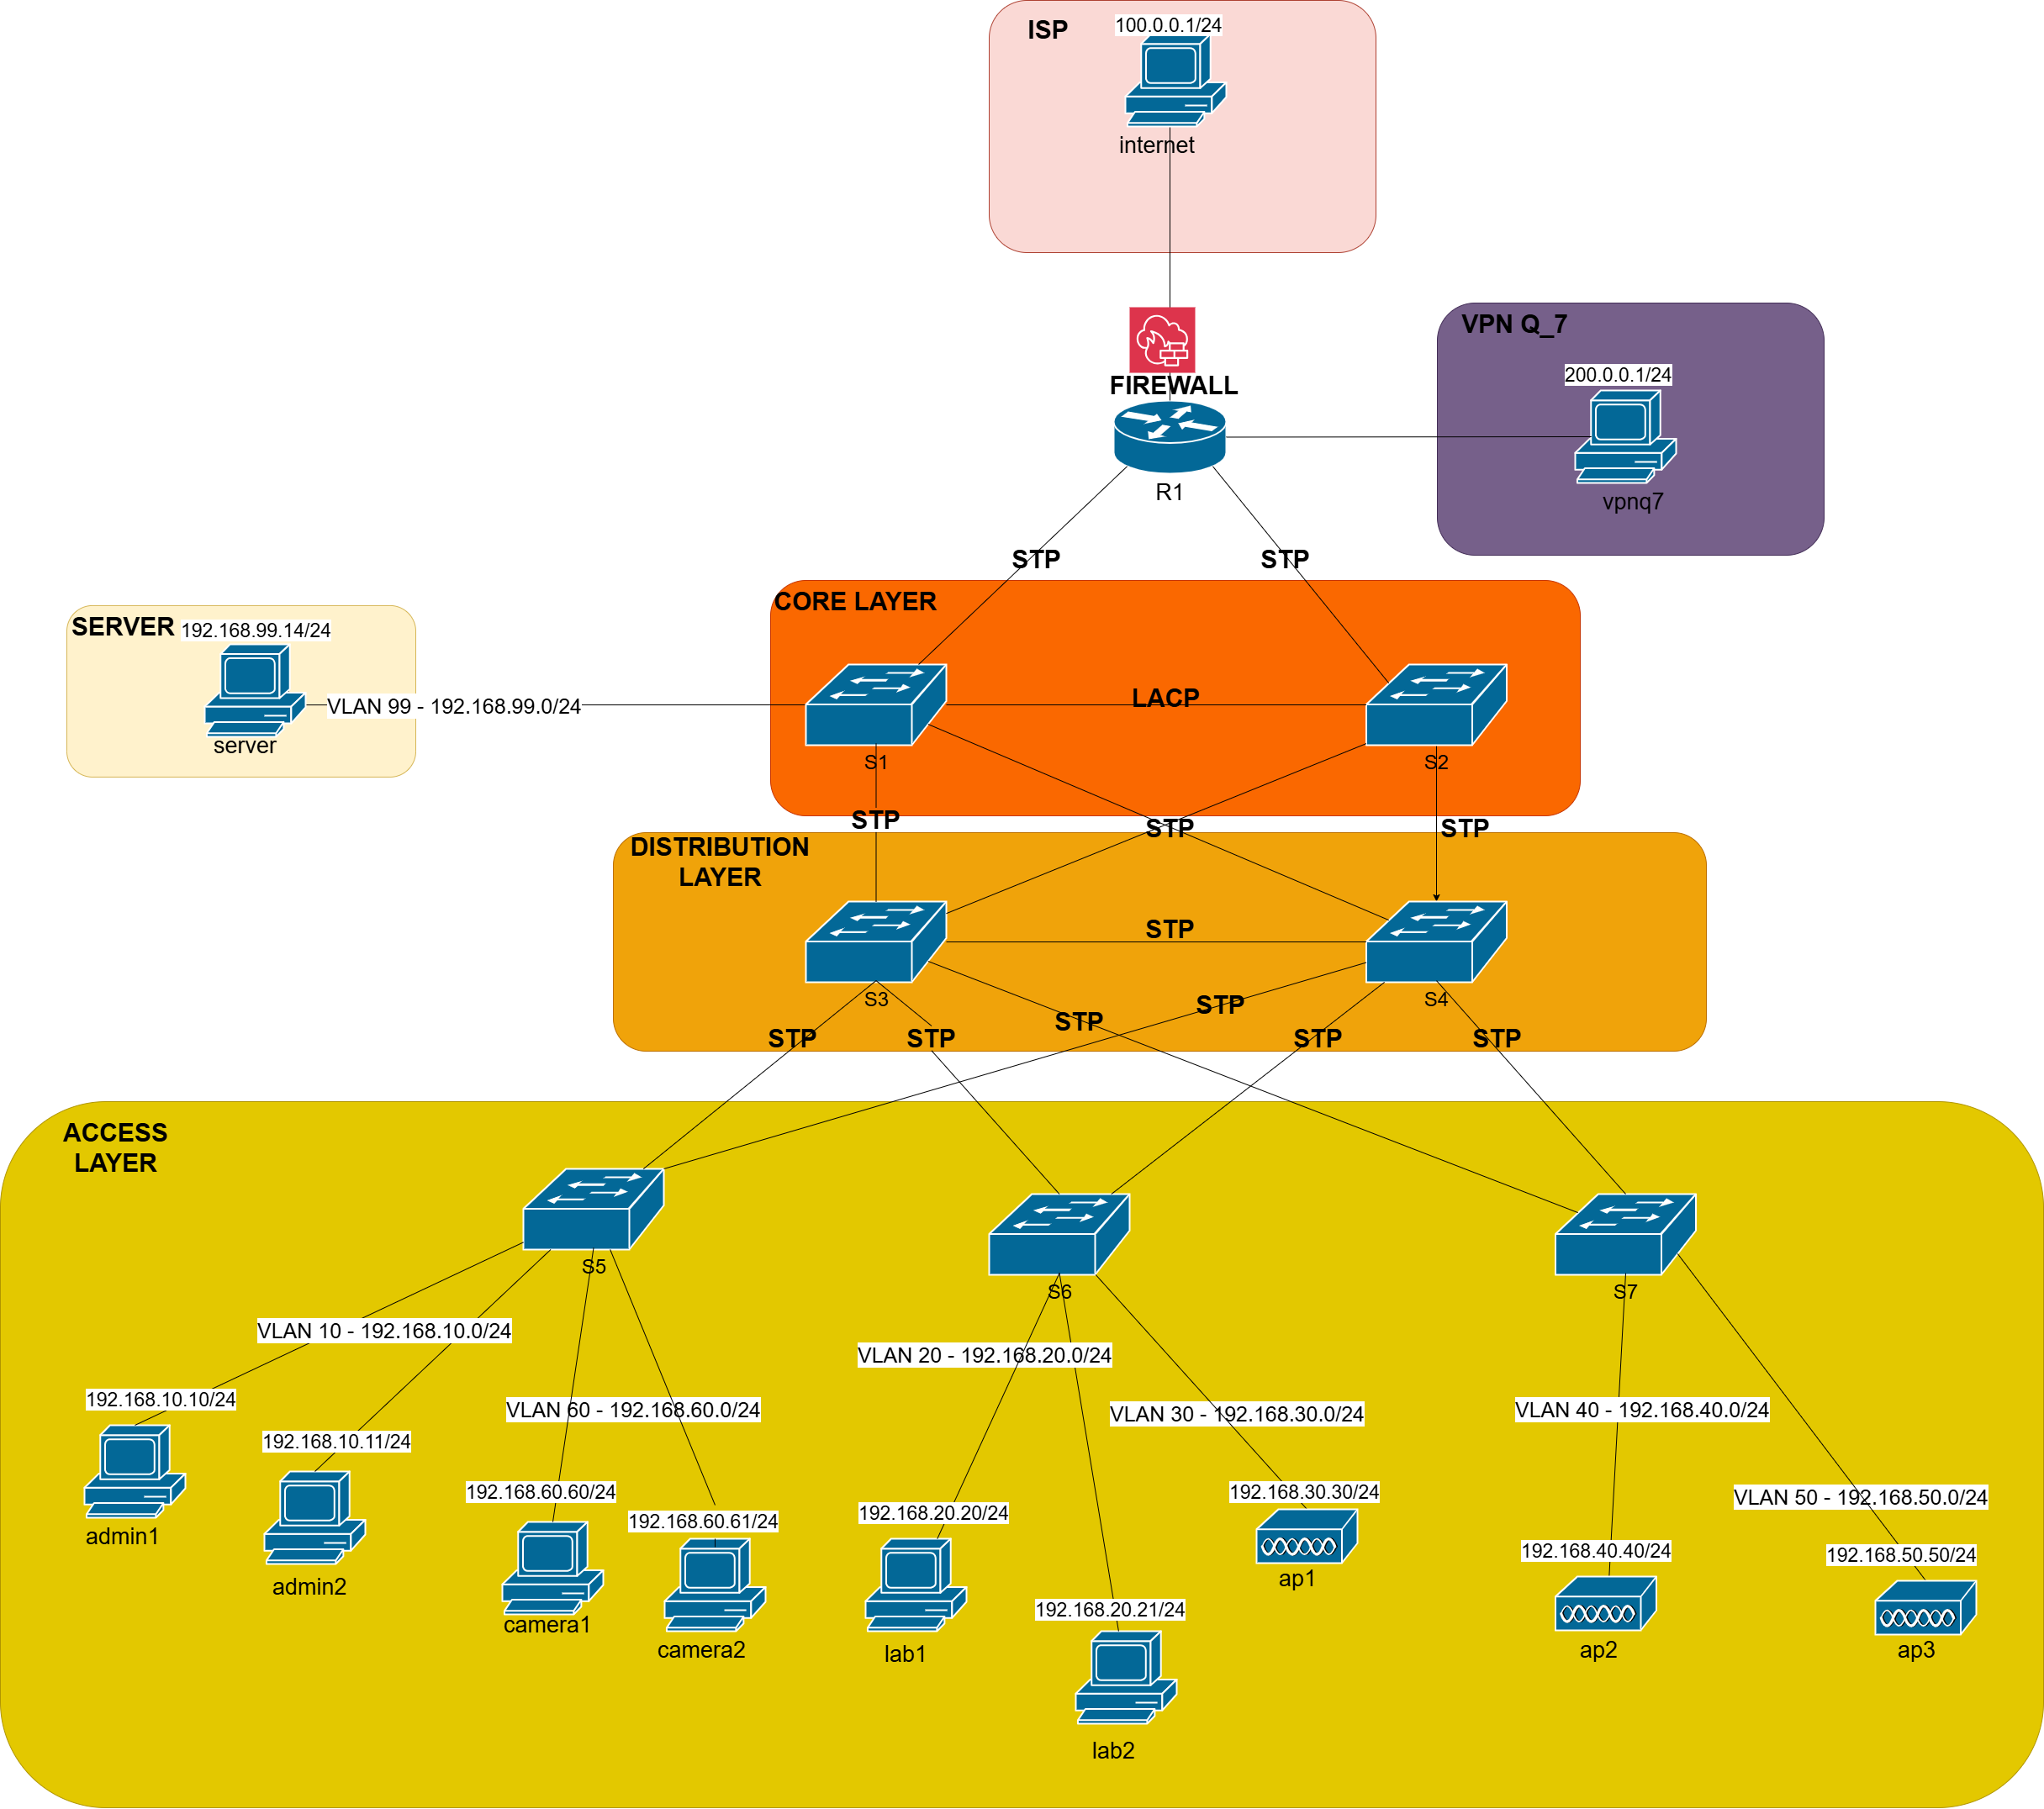
\includegraphics[width=0.9\linewidth]{image/logical_topology.png}
    \caption{Sơ đồ Logic mạng Cơ sở Bảo Lộc với cơ chế dự phòng}
    \label{fig:logical_topo}
\end{figure}

\begin{itemize}
    \item \textbf{Core Layer (Lớp Lõi):} Sử dụng 02 Switch L3 chạy cơ chế dự phòng (HA). Chịu trách nhiệm chuyển mạch tốc độ cao và định tuyến giữa các VLAN.
    \item \textbf{Distribution Layer (Lớp Phân phối):} Đặt tại từng tòa nhà (Tòa A, Tòa B). Thực hiện gom lưu lượng từ các tầng và áp dụng các chính sách ACL/Security.
    \item \textbf{Access Layer (Lớp Truy cập):} Các Switch L2 kết nối trực tiếp đến PC, Wifi AP và Camera. Hỗ trợ PoE để cấp nguồn cho thiết bị.
\end{itemize}

\subsection{Quy hoạch IP và VLAN (IP Addressing Plan)}
Hệ thống sử dụng dải mạng Private `10.20.0.0/16` dành riêng cho Cơ sở Bảo Lộc để tránh trùng lặp với Trụ sở chính.

\begin{table}[H]
\centering
\begin{tabularx}{\linewidth}{|c|l|l|X|}
\hline
\textbf{VLAN ID} & \textbf{Tên VLAN} & \textbf{Subnet} & \textbf{Mục đích sử dụng} \\ \hline
10 & Management & 10.20.10.0/24 & Quản trị thiết bị mạng (Switch, AP, Firewall). \\ \hline
20 & Faculty & 10.20.20.0/24 & Dành cho Giảng viên và Cán bộ nhân viên. \\ \hline
30 & Student & 10.20.30.0/24 & Dành cho Sinh viên (Phòng Lab, Thư viện). \\ \hline
40 & Wireless & 10.20.40.0/22 & Dành cho mạng Wifi (Subnet lớn /22 hỗ trợ 1000 IP). \\ \hline
50 & Server & 10.20.50.0/24 & Server Farm (Web, Mail, DNS nội bộ). \\ \hline
99 & IoT/Camera & 10.20.99.0/24 & Hệ thống Camera an ninh và thiết bị IoT. \\ \hline
\end{tabularx}
\caption{Bảng quy hoạch VLAN và IP}
\label{tab:vlan_ip}
\end{table}

\subsection{Giải pháp Kỹ thuật và Dự phòng}
Dựa trên tiêu chí "Sẵn sàng" (Availability) có trọng số cao, các công nghệ sau được áp dụng:

\begin{enumerate}
    \item \textbf{Dự phòng Gateway (FHRP):} Sử dụng giao thức \textbf{VRRP} hoặc \textbf{HSRP} giữa 2 Core Switch. Nếu Core 1 hỏng, Core 2 sẽ tự động nhận làm Gateway ảo (Virtual IP) mà không làm gián đoạn kết nối của người dùng.
    \item \textbf{Dự phòng Liên kết (Link Aggregation):} Sử dụng \textbf{LACP (802.3ad)} để gộp nhiều đường dây vật lý thành 1 đường logic, vừa tăng băng thông vừa dự phòng đứt dây.
    \item \textbf{Định tuyến (Routing):} Sử dụng giao thức định tuyến động \textbf{OSPF} để kết nối về Trụ sở chính qua đường truyền VPN/Leased Line.
    \item \textbf{Bảo mật Zero Trust:} 
    \begin{itemize}
        \item Áp dụng \textbf{Port Security} tại lớp Access để chống cắm dây lạ.
        \item Tách biệt hoàn toàn VLAN Camera và VLAN Sinh viên bằng ACL tại lớp Distribution.
    \end{itemize}
\end{enumerate}